\documentclass[varwidth=true, border=2pt]{standalone}
\usepackage{amsmath,scalerel}

\DeclareMathOperator*{\Bigcdot}{\scalerel*{\cdot}{\bigodot}}
\usepackage{tkz-euclide}
\usetikzlibrary{angles,quotes}

\begin{document}
\usetkzobj{all}
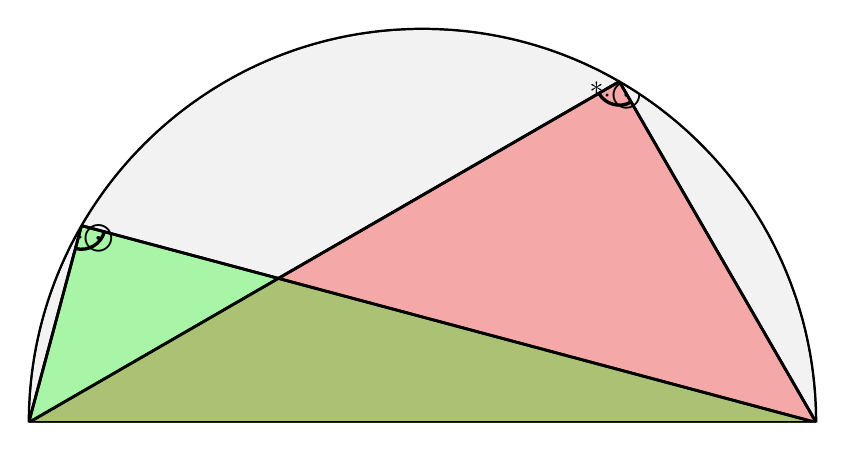
\begin{tikzpicture}
    \tkzSetUpPoint[shape=circle,size=10,color=black,fill=black]
    \tkzSetUpLine[line width=1]
    \tkzDefPoints{0/0/O, -5/0/A, 5/0/B, 5/5/M, -5/5/N}
    \tkzDefPoint(60:5){X}
    \tkzDefPoint(150:5){Y}

    \tkzDrawArc[color=black, thick, fill=gray!10](O,B)(A)

    % Avoid too long edges of polygon
    \tkzClipPolygon(A,B,M,N)
    \tkzClipCircle(O,B)

    % Draw polygons and mark right angle
    \tkzDrawPolygon[fill=red,fill opacity=0.3](A,B,X)
    \draw pic[very thick, draw, angle radius=3mm,"$\Bigcdot$",angle eccentricity=.6]{angle= A--X--B};

    \tkzDrawPolygon[fill=green,fill opacity=0.3](A,B,Y)
    \draw pic[very thick, draw, angle radius=3mm,"$\Bigcdot$",angle eccentricity=.6]{angle= A--Y--B};

    % lines should not colored
    \tkzDrawPolygon(A,B,X)
    \tkzDrawPolygon(A,B,Y)

    \tkzDrawArc[color=black, thick](O,B)(A)
\end{tikzpicture}
\end{document}